\chapter{Numerical Simulation of Unsteady Laminar Flow}
\section{Problem Description}
\subsection{Governing Equations} % homogenous fluid region, and porous region

\subsection{Boundary Conditions} % Including interface between the homogeneous fluid and porous medium regions


\section{Numerical Methods}
\subsection{Discrete Methods of Time and Space}
\subsection{Solver} % SIMPLE
\subsection{Mesh Generation and Independence Analysis}
The flow domain is chosen to be a square with length of side 60. In order to obtain the fluid state of both inner and outer of the cylinder, the flow domain is divided into three blocks two of whom are in the cylinder and the other is out, as described in Figure \ref{fig: grid}. The grid size is shown in Table \ref{tab: grid}. The Reynolds number and the Darcy number are 100 and 0.0001 separately.



\begin{figure}[]
	\centering
	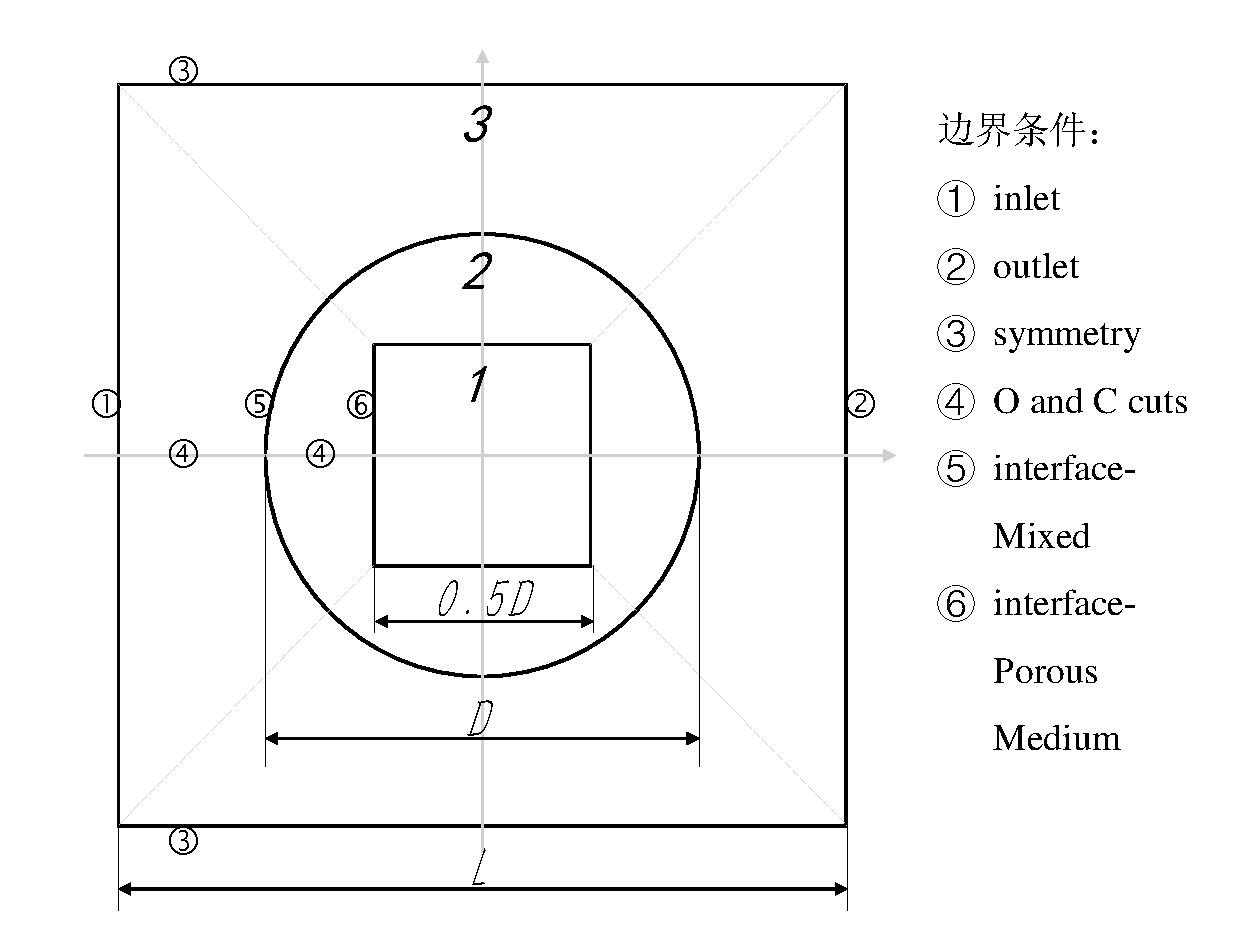
\includegraphics[scale=.6]{../diagrams/grid}
	\caption{The partition of grid blocks.}\label{fig: grid}
\end{figure}
\begin{table}[]
	\centering
	\caption{Grid size.}
	\label{tab: grid}
	\begin{tabular}{@{}cccccc@{}}
		\toprule
		\multicolumn{2}{c}{Blocks}  & Block 1  & Block 2   & Block 3 & Mean drag coefficient    \\ \midrule
		\multirow{4}{*}{Grid size} 
		& Case 1 & 40 $\times$ 40 & 160 $\times$ 25 & 160 $\times$ 140   & 1.2354 \\
		& Case 2 & 60 $\times$ 60 & 240 $\times$ 30 & 240 $\times$ 170   & 1.2426 \\
		& Case 3 & 80 $\times$ 80 & 320 $\times$ 40 & 320 $\times$ 200   & 1.2462 \\
		& Case 4 & 100 $\times$ 100 & 400 $\times$ 50 & 400 $\times$ 230 & 1.2417 \\
		\bottomrule
	\end{tabular}
\end{table}


\section{Summary}
